% ============================================================
% III. PHƯƠNG PHÁP
% ============================================================
\section{Phương pháp}

\begin{frame}{III-A. Mục tiêu và phạm vi baseline}
  \begin{block}{Tại sao chọn BiSeNet?}
    Kiến trúc lightweight kinh điển, tách riêng spatial detail và semantic context $\to$ phù hợp để phân tích mất mát local detail trên thực phẩm fine-grained \cite{bisenet}
  \end{block}
  \vspace{0.3em}
  \textbf{Ba mục tiêu thiết lập baseline}
  \begin{enumerate}
    \item \textbf{Mốc hiệu năng}: điểm tham chiếu rõ ràng trên không gian nhãn gốc 103 lớp
    \item \textbf{Kiểm tra giới hạn}: BiSeNet suy giảm ra sao với ranh giới yếu và texture phức tạp
    \item \textbf{Chuẩn hóa pipeline}: quy trình huấn luyện/đánh giá đồng nhất để so sánh công bằng
  \end{enumerate}
  \vspace{0.3em}
  % \begin{alertblock}{Phạm vi}
  %   Baseline được huấn luyện \textbf{trực tiếp} trên \texttt{FoodSeg103} nguyên thủy (103 lớp), \textbf{không} áp dụng bất kỳ bước gộp hoặc tái cấu trúc nhãn nào. Thực nghiệm tái cấu trúc nhãn (103 $\to$ 75 lớp) là nhánh phân tích \textbf{bổ sung độc lập}, thực hiện sau khi baseline đã hoàn tất.
  % \end{alertblock}
\end{frame}

\begin{frame}{III-B. Kiến trúc BiSeNet}
  \begin{columns}
    \column{0.4\textwidth}
      \begin{itemize}
        \item \textbf{Spatial Path}: 3 conv stride-2 $\to$ $\frac{1}{8}$ ảnh gốc, bảo toàn chi tiết cạnh và texture
        \item \textbf{Context Path}: Xception39 + GAP $\to$ trường thụ cảm rộng
        \item \textbf{ARM}: channel-wise attention tinh lọc đặc trưng context
        \item \textbf{FFM}: nối hai luồng + SE-like reweighting
      \end{itemize}
    \column{0.59\textwidth}
      \begin{figure}
        \centering
        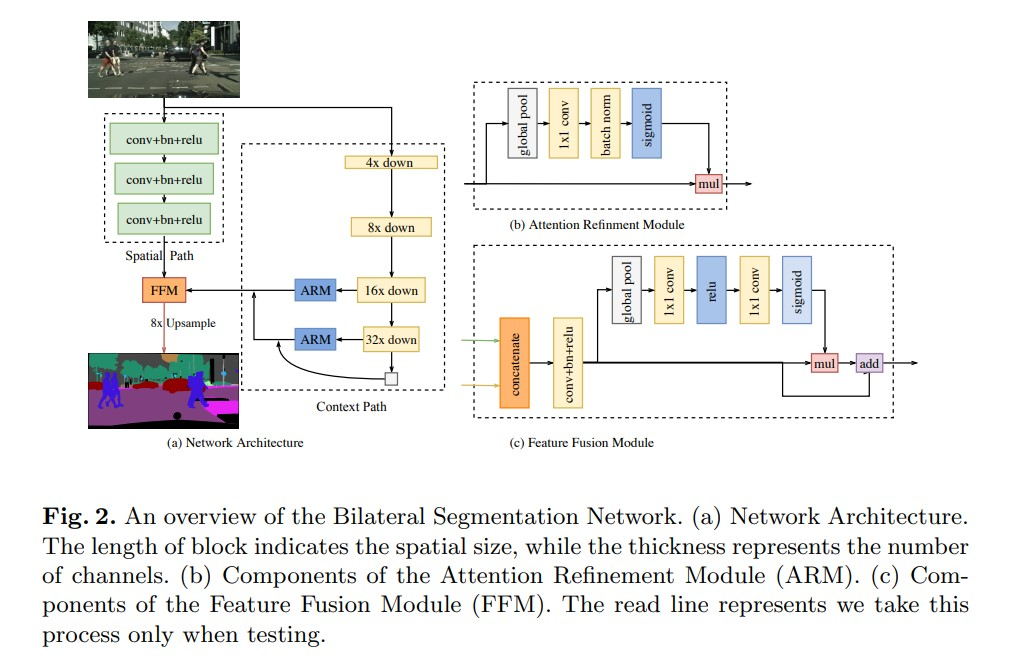
\includegraphics[width=\linewidth]{img/report/BiSeNET-architecture.jpg}
        % \caption{Kiến trúc BiSeNet}
      \end{figure}
  \end{columns}
\end{frame}

\begin{frame}{III-C. Hàm mất mát cho baseline}
%   \begin{columns}
%     \column{0.58\textwidth}
      \textbf{Deep Supervision Loss}
      \[
        \mathcal{L} = \mathcal{L}_p + \alpha\mathcal{L}_2 + \alpha\mathcal{L}_3,\quad \alpha=1
      \]
      Ba thành phần đều dùng pixel-wise softmax cross-entropy:
      \[
        \mathcal{L}_o = -\frac{1}{|\Omega|}\sum_{(i,j)\in\Omega}\log p^{(o)}_{i,j,y_{i,j}}
      \]
      \begin{itemize}
        \item Auxiliary losses chỉ dùng khi train, bỏ khi inference.
        \item Mục tiêu: tăng ổn định gradient và cải thiện học đặc trưng ở tầng trung gian.
      \end{itemize}
    % \column{0.38\textwidth}
      \begin{block}{Vì sao chọn Cross-Entropy?}
        \begin{itemize}
          \item đơn giản, ổn định
          \item dễ tái lập kết quả
          \item phù hợp vai trò baseline
        \end{itemize}
      \end{block}
%   \end{columns}
\end{frame}

\begin{frame}{III-D. Cấu hình huấn luyện baseline}
%   \begin{columns}
%     \column{0.46\textwidth}
          \begin{alertblock}{Nguyên tắc}
        Baseline tốt là baseline \textbf{ổn định và giải thích được}, không nhất thiết là điểm số cao nhất.
      \end{alertblock}
      \begin{itemize}
        \item Thiết lập hướng tới \textbf{reproducibility} trước khi tối ưu cực đại.
        \item Giữ cấu hình gọn để so sánh công bằng với các module cải tiến sau này.
      \end{itemize}


    % \column{0.5\textwidth}
      \begin{table}
        \tiny
        \begin{tabular}{ll}
          \toprule
          \textbf{Tham số} & \textbf{Giá trị} \\
          \midrule
          Crop size    & $512\times512$ \\
          Backbone     & Xception39 \\
          Optimizer    & SGD mom=0.9 \\
          Init LR      & $2.5\times10^{-2}$ Poly \\
          Batch size   & 8 \\
          Epochs       & 150 \\
          Aug scales   & \{0.75, 1.0, 1.5, 1.75, 2.0\} \\
          AMP          & True \\
          \bottomrule
        \end{tabular}
        \caption{Cấu hình huấn luyện BiSeNet}
      \end{table}
%   \end{columns}
\end{frame}
